\documentclass[a4paper,11pt]{article}

%\usepackage[pdftex]{graphicx}
\usepackage{amsmath}
%\usepackage[latin1]{inputenc}
%\usepackage{hyperref}
%\usepackage[T1]{fontenc}
%\usepackage[utf8]{inputenc}
%%GD Quand je mets usepackage[utf8]{inputenc} je n'arrive plus à compiler la biblio
%J'ai essayé de débuger : je n'y suis pas arrivé
\usepackage{rotating}
\usepackage{setspace}
\usepackage{lscape}
\usepackage[round]{natbib}
\usepackage{multirow}
\usepackage{rotating}
\usepackage{vmargin}
\usepackage{epstopdf}
\usepackage{hyperref}
\usepackage{float}
\usepackage{caption}
\usepackage[tableposition=top]{caption}
\usepackage{amsfonts}
\usepackage{bbold}
\usepackage{bbm}
\usepackage[flushleft]{threeparttable}
%\usepackage{bbold}
%\usepackage[T1]{fontenc}
% JH : impossible de compiler avec le package bbold, remplacé par amsfonts
% LP : impossible de compiler avec le package bbold, remplacé par bbm
\usepackage{upgreek}
\usepackage{comment}
\includecomment{commentGD}
\usepackage[draft]{todonotes}
%\usepackage[disable]{todonotes}
%%GDPour cacher les notes, \usepackage[disable]{todonotes}

\usepackage{setspace}

%\usepackage[nolists, figuresfirst]{endfloat}
%\usepackage{sidefloat}

\setlength{\abovecaptionskip}{-8pt}

%\usepackage[usenames]{color}
%\definecolor{grey}{rgb}{0.35,0.35,0.35}
%\definecolor{webdarkblue}{rgb}{0,0,0.4}
%\definecolor{orange}{rgb}{0.7,0.2,0.05}


%\usepackage[pdfcreator={PDFLaTeX}, pdfproducer={PDFLaTeX}, pdfstartview=FitH, pdfpagemode=UseOutlines, pagebackref=false, colorlinks={true},
%citecolor={webdarkblue}, linkcolor={webdarkblue},
%urlcolor={webdarkblue}]{hyperref}



%\addtolength{\oddsidemargin}{-0.4in}
%\addtolength{\evensidemargin}{-0.4in}
%\addtolength{\textwidth}{0.8in} \addtolength{\topmargin}{-0.85in}
%\addtolength{\textheight}{1.7in}
\renewcommand{\baselinestretch}{1.2}

\newcommand\cites[1]{\citeauthor{#1}'s\ (\citeyear{#1})}

\newcommand\citeh[1]{\citeauthor{#1}'\ (\citeyear{#1})}

\setmarginsrb{3cm}{2cm}{3cm}{2cm}{0,5cm}{0,5cm}{0,3cm}{0,5cm}



% commands

\newcommand{\bi}{\begin{itemize}}
\newcommand{\ei}{\end{itemize}}
\newcommand{\be}{\begin{enumerate}}
\newcommand{\ee}{\end{enumerate}}
\newcommand{\bd}{\begin{description}}
\newcommand{\ed}{\end{description}}
\newcommand{\beqa}{\begin{eqnarray}}
\newcommand{\eeqa}{\end{eqnarray}}
\newcommand{\beq}{\begin{equation}}
\newcommand{\eeq}{\end{equation}}
\newcommand{\bs}{\bigskip}
\newcommand{\A}{$^a$}
\newcommand{\B}{$^b$}
\newcommand{\C}{$^c$}

\renewcommand{\baselinestretch}{1.2}
%\doublespacing

%\linespread{1.6}

%\newcommand{\note}[1]{\footnote{\begin{doublespace}#1\end{doublespace}}}


\begin{document}


\title{\textsc{International Transport costs:\\New Findings from modeling additive costs} \\
Answer to Referee 1}

\author{Guillaume \textsc{Daudin}\thanks{%
Université Paris-Dauphine, PSL University, CNRS, 8007, IRD, 260, LEDa, DIAL, 75016, Paris, France ; email: \url{guillaume.daudin@dauphine.psl.eu}}  \qquad J\'{e}r\^{o}me \textsc{H\'{e}ricourt} \thanks{Universit\'{e} de Lille - LEM-CNRS UMR 9221, France \& CEPII, France; email: \url{jerome.hericourt@univ-lille.fr}}\qquad Lise \textsc{Patureau}\thanks{Corresponding author.
University Paris-Dauphine \& PSL University, LEDa, 75016 Paris, France;  email: \url{lise.patureau@dauphine.psl.eu} } }


\date{September 2021}
 \maketitle
\bigskip

We would like to thank you for your insightful comments. They led us to introduce some
significant changes to the paper that we hope address your concerns. We first give you an overview
of the revision (Section \ref{sec:main_changes}) before answering in detail each of your comments (Section \ref{sec:detailed_answers}). Number of sections, pages and equations mentioned in the text refer to the revised version. When necessary, we refer to number of sections, pages and equations from the submitted version. In this case, they are written between brackets.

\section{Main changes \label{sec:main_changes}}

The structure of the paper has been modified after taking into account the referees' comments.
\begin{itemize}
\item In the submitted version, [Section 2] was devoted to the estimation of international transport costs; specifically, their break-down in two components, additive and ad-valorem. In [Section 3], we investigated the role of additive costs in the decomposition of transport costs time trends, between structural changes and composition effects. [Section 4] was devoted to the robustness analysis relative to the results from both previous sections.
\item In the revised version, we have strengthened the robustness checks regarding the estimation results of international transport costs (robustness checks to aggregation and to endogeneity have been added). Accordingly, the previously-called [Section 2] has been split in two Sections: Section 2, where we present the data and the estimation strategy; and Section 3, which presents the results and now includes the robustness checks as a final sub-section. For sake of brevity, the robustness analysis related to composition effects has been sent to the Appendix (Section C.3).
\item Both referees asked us to highlight the implications of additive costs (the ``Big Picture''). We agree that this was not enough emphasized in the submitted version, and we thank the referees for their suggestions on that issue. The revised version answers this concern in two points.
    \begin{enumerate}
    \item We maintain the analysis of the transport costs time trends (previously [Section 3], now Section 4); but we improved this section’s readibility by leaving the technical aspects in the Appendix (Section C). As such, we hope that the main message of this Section is easier to understand.
    \item Most importantly, we now emphasize the ``Big Picture'' welfare implications of additive costs on theoretical grounds. Through the lens of the \cites{melitz} model amended to integrate additive costs, we analyze the welfare gains that derive from the reduction in international transport costs that we have estimated in Section 3, to quantify the extra welfare gains attributable to the reduction of their additive component. This analysis is conducted in a new Section 5.
        \end{enumerate}
\item To keep the paper (both the main text and with appendix included) within a reasonable number of pages, yet to be fully transparent about our results, we have added numerous detailed tables to the Online Appendix.
\end{itemize}

We now answer in detail each of your comments given in italics.

\section{Detailed answers \label{sec:detailed_answers}}


\subsection{Critique 1: Empirical Strategy}

\textit{Using the notation of the authors, they are interested
in identifying the share of the specific cost in the total transport cost. Namely,}
\begin{eqnarray*}
&& \frac{\frac{t_{is(k)}}{\tilde{p}_{ik}}}{\tau_{is(k)}-1 + \frac{t_{is(k)}}{\tilde{p}_{is(k)}}} \\
\text{or,} &&\frac{t_{is(k)}}{(\tau_{is(k)}-1)\tilde{p}_{is(k)} + t_{is(k)}}
\end{eqnarray*}

\textit{The way they approach the problem is that they assume that (a) $\tau_{ik} = \tau_i\tau_{k}$,
(b) $t_{ik} = t_i +t_k$, and (c) $t_k$ and $\tau_k$ are uniform across products within industry
s. After imposing these assumptions, they estimate the following specification}

\begin{equation}
\ln\left(\frac{p_{ik}}{\widetilde{p}_{ik}}-1 \right)= \ln \left(\tau_{i} \times \tau_{s(k)} -1+\frac{t_{i} + t_{s(k)}}{\widetilde{p}_{ik}} \right) + \epsilon_{ik} \label{eq:equation0}
\end{equation}

\textit{in which $\tau_i$, $\tau_{s(k)}$, $t_i$, and $t_{s(k)}$ are identified as fixed effects coefficients.
In my opinion this choice of strategy is quite sub-optimal, as (i) it relies on
the strong assumptions highlighted above, (ii) it is computationally expensive
as noted by the authors on multiple occasions, and (iii) it is subject to an
endogeneity problem, which the authors disregard with one sentence, but which
is rather detrimental in my opinion.}


%\paragraph{Strategy of answer} To clarify the discussion, we decided to answer concerns (i) and (iii) each in turn. As regards to point (ii), we run the referee's proposed estimation method without relying on instrumental variables; this way, the results are comparable with the benchmark results, the only change being the estimation strategy (Section \ref{subsec:functional_form} of the letter). As noted above, this drove us to maintain our estimation method as benchmark. As regards to point (iii), we instrument fas prices at the $k=$ 10-digit level, still based on our original estimation strategy (but switching to a finest product category disaggregation level $k=10$). This allows a direct comparison of the results obtained in the non-linear least squares regression with those obtained with IV (with $s=3$ digit at the sector level and $k=10$ at the product level in both cases). This is developed in \textbf{Section ??? of the letter}.


These three points indeed deserve careful consideration. We provide separate answers to each of them below.

%\subsubsection{On the justifications for our empirical approach}

\subsubsection{Concern (i): About the assumption of separability}
Our main empirical equation and its underlying assumptions regarding the separability of transport costs between their country- and product-level components draw on the one proposed by \citet{Irrazabal_2015} to estimate the share of additive costs in a firm-level context. It relies on a simple theoretical framework with minimal assumptions, and is compatible with most approaches within the so-called category of ``New Trade Theories''.

Further, we provide a robustness check for this separability assumption that $\tau_{ik} = \tau_i\tau_{k}$ and
 $t_{ik} = t_i +t_k$ in Section 3.3.1 of the paper (Table 2 and \textbf{Figure XXX}) \textbf{XXX CHECK AT THE END XXX}). We check the robustness of our results by re-running the estimation without the separability assumption. This comes at the cost of a substantial increase in the number of fixed in the regression. In 2019, for example, there are 14,016 country$\times$sector pairs. Adding 28,032 fixed effects (number of country pairs $\times2$ for the two additive and multiplicative costs fixe effects) rather than ``only'' 836 ($(188+230)\times 2$). This is computationally not tractable.
% use "/Users/guillaumedaudin/Documents/Recherche/2013 -- Trade Costs -- local/data/hummels_tra.dta", clear
% keep if year==2019
% keep if mode=="ves"
% gen sector=substr(sitc2,1,3)
% gen blouk = iso_o+sector
% codebook blouk
 For this reason, we have decided to run the robustness check on a reduced sample. For each year, we select the largest exporters that form together at least 80\% of annual trade and the largest traded sectors that form together at least 80\% of annual trade.
 We keep in the sample all trade observations from these exporters and in these sectors.
 This sample is smaller in terms of observations (2,125 for Air, 5,260 for Vessel on average over the period 1974-2019 (see Table 2), vs more than 30,000 on the complete sample, see Table 1). It yet remains quite large in terms of trade coverage (mean of 68\%).\footnote{In the restricted sample at the 3-digit level, we have 25 sectors from 14 countries for Air transport, vs 212 sectors from 190 countries in the large sample; and 54 sectors from 20 countries for Vessel, vs 667 sectors from 192 countries in the complete sample). The vast majority of US imports comes from a selected range of countries, in a selected range of sectors.} On this reduced sample, we re-run the estimation with and without the separability assumption. The results are reported in Section 3.3.1 (Table 2 and \textbf{Figure XXX}). \textbf{XXX CHECK AT THE END XXX}) As we conclude at the end of this section, the trend pattern of the share of additive cost are very similar whether estimated under the separability assumption or not.
 % use "/Users/guillaumedaudin/Documents/Recherche/2013 -- Trade Costs -- local/results/comparaisons_various/stats_comp_baseline_non_séparé.dta", clear
% gen cover = cover_non_séparé/cover_baseline
% sum cover


\subsubsection{Concern (ii): On the use of non-linear least squares (NLS)} As noted by the referee (and in the paper), it is true that relying on the non-linear least squares method is highly demanding computationally when the number of fixed effects is high. This constraint notably drove us to impose the separability assumption and retain $s=3$ as the relevant sectoral degree of aggregation.


The referee writes: \textit{A more natural approach is what the authors, at some point, refer to as the Hummels' Methodology. That is, one can alternatively estimate the share of the additive component as:}
$$\frac{t_{ik}}{ (\tau_{ik}-1)\tilde{p}_{ik} + t_{ik}} = \beta_{ik}$$

\textit{where $\beta_{ik}$ is the elasticity of transport costs w.r.t. unit price. Given the authors' objective and the data they are using, $\beta$ can be separately estimated for each industry-country pair using the following regression:}

\begin{equation}
\ln f_{ikd} = \beta_{is(k)}\ln \tilde{p}_{ikd} + \text{Controls}_{ikd} +\epsilon_{ikd} \label{eq:estimation_ref1}
\end{equation}

\textit{where $d$ denotes the US district of entry and $k$ denotes an HS10 product} ($f_{ikd}$ being the transport costs). \textit{The
identification of $\beta_{ik}$, in this case, would rely on the across HS10 product and
district-of-entry variation in $f_{ik}$ and $p_{ik}$. Estimating the above equation would
obviously require that the authors do not aggregate up the raw Census data
across all districts and all 10-digit products pertaining to the same 5-digit category. [...] The first advantage of this so-called Hummels' approach is that the above regression can be estimated separately for various country-industry pairs, without imposing Assumptions (a) and (b) outlined above.}

\textbf{Our answer:} First of all, we thank the referee for suggesting to improve the comparison between our method and Hummels's one. We took this remark into account by adding a new sub-section in the revised version (Section 2.2, paragraph ``Estimation strategy'' \textbf{XXX Check XX}). As we now show in this Subsection, the elasticity of transport costs to unit prices $\beta_{is(k)}$ (in absolute value) also corresponds to the share of additive costs in total transport costs. The share of additive costs can hence be uncovered by regressing transport costs on unit fas prices, along the lines you suggest.

Now coming to the technical side, we thank the referee for his/her relevant suggestion of an alternative estimation method. This drove us to question our own empirical specification deeper. In the end, we decided to maintain our empirical strategy in the revised version, because its advantages seem to overweight the possible costs, and the alternative that the referee suggests does not go without a few important limitations. We develop each line of argument in our answer. Yet, because the referee's estimation method is also an interesting alternative, we added a new section in the Online appendix devoted to it (Section D.3 \textbf{XXX CHECK XXX }). After reading our answer, we hope to convince you that we made the right choice.


\paragraph{Estimating the share of additive costs: Highlighting some requirements} Our estimated equation relies on non-linear estimation methods, such as Non-Linear Least Squares. However, even with another formulation, such as the one suggested by the referee in Equation (\ref{eq:estimation_ref1}), we would still be constrained to resort to non-linear estimators. This is due to the necessity of imposing an \textit{ex-ante} restriction on parameters, i.e. $\tau \geq 1$ and $t \geq 0$, or $0 \leq  \beta \leq 1$. Should we relax these restrictions, standard linear, least squares estimates often deliver negative, meaningless estimates. In this respect, implementing the referee's method (see below) does not dispose of the requirement of resorting on non-linear estimates (and the computational, time-consuming burden it induces -- though the referee’s method is indeed less computational intensive). Imposing this parameters constraint was not made clear enough in the initial version, and we did our best to make this very important justification clearer in the revised version, as it is now exposed in footnote 12 page 8. \textbf{XXX Verifier à la fin? GD XXX }\smallskip



\paragraph{Exploring Referee's alternative functional form \label{subsec:functional_form}}

The estimation strategy suggested by the referee starts from Equation (\ref{eq:Hummels}) linking transport costs and unit prices as assumed in Hummels (2007), yielding Equation (\ref{eq:estimation_ref1}) as estimation equation. By year and transport mode, this implies running the estimation for each country of origin $i$ and each sector $s(k)$ = 3 digit sector, exploiting the variability between sub-sectors at the 10-digit level ($k$) and between ports of entry in the US ($d$).

Despite its interest, implementing the referee's method uncovers some drawbacks, that in our view outweighs those of our method (in particular associated with \textit{Assumptions (a) $\tau_{ik} = \tau_i\tau_{k}$, and (b) $t_{ik} = t_i+ t_{k}$.}) Our answer can be articulated in two steps. First, we challenge the advantages that the referee's estimation method would bring in comparison with our's. Second, we emphasize the drawbacks induced by this method. \smallskip
%
%\paragraph{What we do}
%
%Our estimated equation is written as Equation (\ref{eq:equation0}) with $s$= 3 (or 4) digit and $k$=5 digit (based on Hummels' original dataset from 1974-2004). We thus exploit the variability of transport costs between countries and between 3-digit sectors (conditional on a year and a transport mode, air or vessel). To sum up our methodology:
%\begin{itemize}
%\item Estimating Equation \ref{eq:equation0} provides us with estimates of $\hat{t}_i$, $\hat{t}_{s(k)}$, $\hat{\tau}_i$, $\hat{\tau}_{s(k)}$.
%\item We rebuild
%\begin{eqnarray*}
%\hat{t}_{is(k)} &= &\hat{t}_{i}+\hat{t}_{s(k)} \\
%\hat{\tau}_{is(k)} &= & \hat{\tau}_{i}\times\hat{\tau}_{s(k)}
%\end{eqnarray*}
%\item We deduce the weighted average value of each component $\bar{t}$, $\bar{\tau}$ by year and transport mode, the weighting scheme being the relative value of the flows for each $i,s$ flow, as well as the median, the maximum and the minimum values.
%\item With this in hand, we can (among other things) obtain the estimated share of additive costs in total transport costs for each $i,k$ flow:
%
%
%$$\hat{\beta}_{ik} = \frac{\frac{\hat{t}_{is(k)}}{\tilde{p}_{ik}}}{\tau_{is(k)}-1 + \frac{t_{is(k)}}{\tilde{p}_{is(k)}}} $$
%\end{itemize}
%
%\paragraph{What the referee suggests to do}
%
%The estimation strategy suggested by the referee starts from Equation (\ref{eq:Hummels}) linking transport costs and unit prices as assumed in Hummels (2007). As shown in Subsection (\ref{ssec:interpret_beta}), the elasticity of transport costs to unit prices $\beta_{ik}$ (in absolute value) also corresponds to the share of additive costs in total transport costs. The share of additive costs can hence be uncovered by regressing transport costs on unit (ie, fas) prices. Specifically, the referee suggests to run the estimation based on Equation (\ref{eq:estimation_ref1}).
%
%Precisely, by year and transport mode, this implies running the estimation for each country of origin $i$ and each sector $s(k)$ = 3 digit sector, exploiting the variability between sub-sectors at the 10 digit level ($k$) and between ports of entry in the US ($d$).\footnote{The referee suggests to run his/her proposed estimation strategy considering sectoral aggregation at the 5-digit level (with $k=10$). We followed his suggestion but considering the 3-digit level. We made this choice in view of being able to compare the pros and cons of the referee's method versus ours. In Hummels' (2007) database, which we use until 2004, the finest degree of classification is at the 5-degree level until 2004. For comparability reasons over time, we adopt the same degree of classification $k=5$ for the following years (based on the original Census dataset). As a result, transport costs are estimated at the 3-digit level as benchmark estimate, exploiting heterogeneity at the 5-digit level (for a given origin country, and conditional on year and transport mode). This has driven us to retain $s=3$ when implementing the referee's method, in view of preserving comparability between both strategies.}


\paragraph{a) The advantages of the referee's method are not as specific to this method as suggested}


\begin{itemize}
\item \textit{The first advantage of this so-called Hummels' Approach is that the above
regression can be estimated separately for various country-industry pairs, without
imposing Assumptions (a) $\tau_{ik} = \tau_i\tau_{k}$, and (b) $t_{ik} = t_i+ t_{k}$.} \\

\textbf{Our answer:}
As already discussed in our letter, the separability assumption does not seem to be a strong assumption. This is based on the conclusion drawn from the robustness check on a reduced sample. If it is smaller in terms of observations, it yet remains quite large in terms of trade coverage, as the selected countries and sectors (at the 3-digit level) constitute 68\% of the total value of flows (on a yearly basis). As we conclude at the end of Section 3.3.1 \textbf{XXX CHECK XXX}, whatever the transport mode and for both types of transport costs, the trend patterns of international transport costs are very similar whether estimated under the separability assumption or not.

\item \textit{The second advantage is that there is a handful of previously-proposed instruments (e.g., HS-10 product-specific tariff rates or lagged prices), which the authors can use to overcome the endogeneity problem.}

     \textbf{Our answer:}
We thank the referee for this valuable suggestion. It is worth noticing that we can also handle the instrumentation of fas prices at the HS-10 level with our method - which we do in the revised version.


\item  \textit{The third advantage is that, by adopting this approach, the comparison between the paper [...] and those in Hummels (2007) would become more transparent.}\\
     \textbf{Our answer:}
     We agree with the referee that the comparison with the literature (\citealp{hummels2007} in particular) was not straightforward for the reader in the submitted version. We did our best to make the comparison clearer in the revised version, yet in a way consistent with our estimation method. In contrast to the submitted version, the paper now starts from the relation linking transport costs to the unit price specified in Hummels (2007):
    \begin{equation}
    f_{ikt} = X_{is(k)t}\widetilde{p}_{ikt}^{-\beta_{ikt}} \label{eq:Hummels}
    \end{equation}

     with $f_{ikt} = \frac{p_{ikt}}{\widetilde{p}_{ikt}} -1 $ the transport costs measure, $p_{ikt}$ ($\widetilde{p}_{ikt}$) the cif (fas) price and $\beta_{ikt}$ the price-elasticity of transport costs, with $i$ the origin country, $k$ the product and $t$ for time. As we now show in the paper (Section 2.2), this also corresponds to the share of additive costs in total transport costs:\footnote{For sake of expositional purpose, the reasoning is made without any $i,k,t$ specification in the revised paper. We directly report them here to ease the comparison with the referee's method afterwards.}

     \begin{equation}
     \beta_{ikt} = \frac{\frac{t_{is(k)}}{\widetilde{p}_{ikt}}}{\tau_{is(k)t}-1+\frac{t_{is(k)t}}{\widetilde{p}_{ikt}} } \label{eq:beta_TC}
     \end{equation}

     Equation (\ref{eq:Hummels}) lies at the root of Hummels's (2007) method. In contrast to our method though, \cite{hummels2007} estimates Equation (\ref{eq:Hummels}) on a panel basis and at the sectoral $s(k)$ basis, assuming a mode-specific $\beta$ invariant over time/sector/origin country. Rather than Equation (\ref{eq:Hummels}), this amounts starting from the functional form: $f_{ikt} = X_{is(k)t}\widetilde{p}_{ikt}^{-\beta}$.

     Two alternative strategies are possible. Let us start with our interpretation of the referee's method. It starts from the functional form linking transport costs and the fas price as specified in the Equation (\ref{eq:Hummels}). Taken in log (on a mode/yearly basis), it is written as:
     $$\ln f_{ikd} = \beta_{is(k)}\ln \widetilde{p}_{ikd} +\text{Controls}_{ikd}+ \varepsilon_{ikd}$$

     \noindent with $d$ the district of entry. From this, one can then recover the levels of additive / multiplicative transports costs. Denoting $\widehat{\beta}_{is(k)}$ the estimated $\beta$ for a given sector-country $i,s(k)$, one can indeed solve the following two-equation system:

\begin{eqnarray}
p_{ik} &=& \tau_{is(k)}\widetilde{p}_{ik} +t_{is(k)} \label{eq:system1}\\
\frac{t_{is(k)}}{(\tau_{is(k)}-1)\widetilde{p}_{ik}+ t_{is(k)}} &=& \widehat{\beta}_{is(k)}  \label{eq:system2}
\end{eqnarray}

\noindent with $p_{ik}$ and $\widetilde{p}_{ik}$ the cif and fas prices observed in our dataset (conditional on a given year-transport mode). With two equations and two endogenous variables, the system can be solved.

 Alternatively, our method rather starts from the definition of transport costs as:
     $$\ln f_{ik} = \ln\left(\tau_{is(k)} -1 + \frac{t_{is(k)}}{\widetilde{p}_{ik}}\right) +\varepsilon_{ik}$$
\noindent from which we deduce the additive/multiplicative costs $\widehat{t}_{is(k)}$, $\widehat{\tau}_{is(k)}$ (on a mode/yearly basis). Then, relying on the Hummels's equation, one can deduce the share of additive costs in total transport costs $\beta_{ik}$ through Equation (\ref{eq:beta_TC}), again on a mode/yearly basis.


In this respect, the referee's method and our's are equivalent, in that they both allow to uncover the share of additive costs in total transport costs $\beta$, as well as the value of each trade costs component ($t,\tau$), that vary over time and sectors (and transport mode). Put it differently, our method is consistent with Hummels' methodology - provided that it is adequately reported as such. In comparison with \cite{hummels2007}, one supplementary advantage of our method is that we estimate a $\beta$ that varies over time, origin country and sector. Section 4 ([Section 3] of the submitted version) explores the importance of allowing for such a variability in accounting for the sources of the transport costs time trend. We agree that this was not sufficiently transparent in the submitted version. We hope that the revised version now fits the referee's expectations on this point.

\end{itemize}

As previously noticed, running this estimation limits the time coverage as information is available at the HS-10 level and by ports of entry only since 2001. We have thus run referee's method over the years 2005-2013, at the $s=3, k=10$ sectoral/product levels, and reported the results in the Online Appendix, Section D.3, Table D.1 and Figure D.3.\textbf{XXX Check XXX}\footnote{Notice that we are aware of the referee's suggestion to run his/her estimation strategy considering sectoral aggregation at the 5-digit level (with $k=10$). We yet keep considering sectors at the 3-digit aggregation level, in view of being able to compare the referee's method versus ours.} For sake of reading clarity, we also report here the results of Table D.1 (here Table \ref{tab_comp_referee1_baseline}).

\begin{table}[htbp]
	\caption{Comparison 2005-2013}
	\begin{center}		
		\begin{tabular}{l|cc|cc}
\cline{1-5}
\multicolumn{1}{c}{Transport mode} &
  \multicolumn{2}{|c|}{Air} &
  \multicolumn{2}{c}{Vessel} \\ \hline
Estimation method &
Alternative &
Baseline &
Alternative &
Baseline \\ \hline
Coverage  \\ \hline
\hspace{1em}Nb sectors &
177 &
217 &
203 &
227 \\
\hspace{1em}Nb partners &
112 &
210 &
123 &
204 \\
\hspace{1em}Nb pairs &
3,872 &
12,158 &
3,743 &
12,440 \\ 
\hspace{1em}Annual covered value in Bn U.S. \$ &
262 &
293 &
824 &
906 \\ \hline
\multicolumn{5}{l}{Share of additive costs $\beta$}  \\ \hline
\hspace{1em}Mean &
0.39 &
0.25 &
0.45 &
0.50 \\
\hspace{1em}Median &
0.39 &
0.22 &
0.41 &
0.48 \\
\hspace{1em}Std. dev. &
0.15 &
0.19 &
0.29 &
0.28 \\
\hspace{1em}Time trend coefficient &
-0.012 &
-0.020 &
-0.012 &
-0.031 \\ \hline
%$\beta_{2005}$ &
%  0.41 &
%0.29 &
%0.46 &
%0.53 \\
%$\beta_{2013}$ &
%0.38 &
%0.27 &
%0.44 &
%0.33 \\
%\cline{1-5}
\end{tabular}

		%\begin{tabular}{lllll}
\cline{1-5}
\multicolumn{1}{c}{} &
  \multicolumn{2}{|c}{air} &
  \multicolumn{2}{c}{ves} \\
\multicolumn{1}{c}{} &
  \multicolumn{1}{|r}{Estimating $\beta\_{i,s}$} &
  \multicolumn{1}{r}{baseline} &
  \multicolumn{1}{r}{Estimating $\beta\_{i,s}$} &
  \multicolumn{1}{r}{baseline} \\
\cline{1-5}
\multicolumn{1}{l}{Mean} &
  \multicolumn{1}{|r}{} &
  \multicolumn{1}{r}{} &
  \multicolumn{1}{r}{} &
  \multicolumn{1}{r}{} \\
\multicolumn{1}{l}{\hspace{1em}Nb\_sectors} &
  \multicolumn{1}{|r}{177} &
  \multicolumn{1}{r}{217} &
  \multicolumn{1}{r}{203} &
  \multicolumn{1}{r}{227} \\
\multicolumn{1}{l}{\hspace{1em}Nb\_partners} &
  \multicolumn{1}{|r}{112} &
  \multicolumn{1}{r}{210} &
  \multicolumn{1}{r}{123} &
  \multicolumn{1}{r}{204} \\
\multicolumn{1}{l}{\hspace{1em}Nb\_pairs} &
  \multicolumn{1}{|r}{3,872} &
  \multicolumn{1}{r}{12,158} &
  \multicolumn{1}{r}{3,743} &
  \multicolumn{1}{r}{12,440} \\
\multicolumn{1}{l}{\hspace{1em}Covered trade value} &
  \multicolumn{1}{|r}{2.62e+11} &
  \multicolumn{1}{r}{2.93e+11} &
  \multicolumn{1}{r}{8.24e+11} &
  \multicolumn{1}{r}{9.06e+11} \\
\multicolumn{1}{l}{beta} &
  \multicolumn{1}{|r}{} &
  \multicolumn{1}{r}{} &
  \multicolumn{1}{r}{} &
  \multicolumn{1}{r}{} \\
\multicolumn{1}{l}{\hspace{1em}Mean} &
  \multicolumn{1}{|r}{0.39} &
  \multicolumn{1}{r}{0.25} &
  \multicolumn{1}{r}{0.45} &
  \multicolumn{1}{r}{0.50} \\
\multicolumn{1}{l}{\hspace{1em}Median} &
  \multicolumn{1}{|r}{0.39} &
  \multicolumn{1}{r}{0.22} &
  \multicolumn{1}{r}{0.41} &
  \multicolumn{1}{r}{0.48} \\
\multicolumn{1}{l}{\hspace{1em}Std. dev.} &
  \multicolumn{1}{|r}{0.15} &
  \multicolumn{1}{r}{0.19} &
  \multicolumn{1}{r}{0.29} &
  \multicolumn{1}{r}{0.28} \\
\multicolumn{1}{l}{Time trend} &
  \multicolumn{1}{|r}{} &
  \multicolumn{1}{r}{} &
  \multicolumn{1}{r}{} &
  \multicolumn{1}{r}{} \\
\multicolumn{1}{l}{\hspace{1em}Coefficient} &
  \multicolumn{1}{|r}{-0.025} &
  \multicolumn{1}{r}{-0.046} &
  \multicolumn{1}{r}{-0.143} &
  \multicolumn{1}{r}{-0.063} \\
\multicolumn{1}{l}{beta\_2005} &
  \multicolumn{1}{|r}{} &
  \multicolumn{1}{r}{} &
  \multicolumn{1}{r}{} &
  \multicolumn{1}{r}{} \\
\multicolumn{1}{l}{\hspace{1em}Mean} &
  \multicolumn{1}{|r}{0.41} &
  \multicolumn{1}{r}{0.29} &
  \multicolumn{1}{r}{0.46} &
  \multicolumn{1}{r}{0.53} \\
\multicolumn{1}{l}{beta\_2013} &
  \multicolumn{1}{|r}{} &
  \multicolumn{1}{r}{} &
  \multicolumn{1}{r}{} &
  \multicolumn{1}{r}{} \\
\multicolumn{1}{l}{\hspace{1em}Mean} &
  \multicolumn{1}{|r}{0.38} &
  \multicolumn{1}{r}{0.27} &
  \multicolumn{1}{r}{0.44} &
  \multicolumn{1}{r}{0.33} \\
\cline{1-5}
\end{tabular}

	
{\parbox[l]{12cm}{ \vspace{4pt}\footnotesize{Notes: Time trend coefficient is the annual growth rate.}}}
\end{center}
	\label{tab_comp_referee1_baseline}%
\end{table}%


Regarding the share of additive costs $\beta$, the comparison between the two methods goes in opposite directions depending on the transport mode. While the estimated $\beta$ is lower for maritime transport with the alternative method (also displaying a larger decrease over the period), the opposite holds for Air transport. In any case yet, the share of additive costs remains substantial, around 40\% on average over the period. In this respect, it confirms the main message of our paper shedding light on the importance of the additive component in international transport costs.

Yet, the suggested method does not go without a few important limitations, that we now develop.


\paragraph{b) The referee's method is not without drawbacks}


\begin{itemize}
\item[Concern 1] The suggested estimation strategy implies having much less data to cover.

As noted above, the suggested method implies that the estimation is run at the sector-country level (on top of being mode-year specific), exploiting the variability within each origin country-3d sector pair across 10-d sub-sectors and ports of entry. Yet, it appears that for many couples (country, 3-digit sector), there is too few variability across sub-sectors or ports en entry given the number of fixed effects included in the regression, such that estimation can not be run. This can be seen comparing the number of observations by year/ transport mode with our method / with the referee's method reported in Table \ref{tab_comp_referee1_baseline} (also reported in the online appendix, Section D.3. \textbf{XXX Check XXX}. Put it differently, this methodology discards country-sector pairs that export a limited range of goods to the US and/or which arrive in the USA through the same ports of entry. This may induce a selection bias in the sample covered for estimation. As reported in Table  \ref{tab_comp_referee1_baseline}, if the number of pairs covered is much lower (especially in the list of countries covered), this concern can yet be mitigated by noticing that the covered value of trade flows is only slightly lower. If it reduces the sample of sectors and origin countries covered, this method preserves the majority of trade flows in value.

The most important limitation rather comes from the coverage period. Information about the port of entry are only available since 1989, which is already smaller than our full sample starting in 1974. On top of that, because of the Covid situation, the US Bureau of Census was only able to send them the CDs relative to the years 1997-1999 and 2001-2019. Implementing the referee's method would hence necessarily reduce the time coverage of our analysis by more than 20 years (skipping the 1974-1996 years in particular). In our view, the historical coverage is interesting per se, as it provides useful insights about how transport costs have evolved over time. Eliminating this dimension of the paper would be detrimental to its value-added.


\item[Concern 2] The suggested method features less accuracy in the estimation of the $\beta$.

If we take the value of the $\beta$ by itself, there is no clear criteria to discriminate between the value estimated with our method and the one obtained with the suggested method (when, of course, run on the same sample). Further, as shown in Table \ref{tab_comp_referee1_baseline}, no clear conclusion on a potential upwards or downwards bias that would be attached to our method. Things are more clear-cut in terms of accuracy of the estimation. Specifically, our method yields a more precise estimation of the $\beta$ than the referee's method. To develop on this, for each year and transport mode:
    \begin{itemize}
    \item With the referee's method, we estimate one value for the share of additive component $\beta$ at the $i,s$ level denoted $\hat{\beta}^{ref}_{is(k)}$ associated with a standard deviation $SD_{is}$, by year and transport mode. From this, we can approximate the 5-95\% threshold values through:
        $$\hat{\beta}_{is}^{min,ref} = \hat{\beta}^{ref}_{is(k)} - 1.96 SD_{is},\quad \hat{\beta}_{is}^{max,ref} = \hat{\beta}^{ref}_{is(k)} + 1.96 SD_{is}$$

        From this, we can deduce the confidence interval $CI^{ref}_{is} = \hat{\beta}_{is}^{max,ref} - \hat{\beta}_{is}^{min,ref}$.

        \item  Our method provides estimates of the underlying trade costs components ($\widehat{\tau}_i$, $\widehat{\tau}_s$, $\widehat{t}_i$, $\widehat{t}_s$) with an associated matrix of variance-covariance, from which we can rebuild $\beta_{is}$ (on a year-transport mode basis). As such, it does not yield an estimate of $\beta_{is}$ and an associated standard deviation, so that we cannot directly compare the precision of the estimation. We then deduce the accuracy of the $\beta$ estimate by relying on bootstrap method. Specifically, on a yearly/mode basis we draw a distribution of trade costs components and associated $\beta_{is}$ (10,000 random draws) from which we can compute the mean, the median and the 5-95 threshold values for each couple $i,s$. Noticing $\beta_{is}^{95}$ and $\beta_{is}^{05}$ the associated thresholds, we then obtain the confidence interval $CI_{is}= \beta_{is}^{95}- \beta_{is}^{05}$.\footnote{Notice that this should be made on the same sample as the one obtained with the referee's method, since the goal is to compare the accuracy of the $\beta_{is}$ estimate - implying to have the same sample of countries / sectors at first. }



    \item We can then evaluate the accuracy of each estimation method by comparing the size of the confidence intervals of the $\beta$, for each couple $i,s$ (by year and transport mode). We summarize this comparison in Figure \ref{fig:accuracy_beta}, which reports the distribution of the ratio of confidence intervals, taken in log.


    \begin{figure}[htbp]
    \caption{Accuracy of the estimation of the $\beta$: Comparison}
    \label{fig:accuracy_beta}
    \begin{center}
    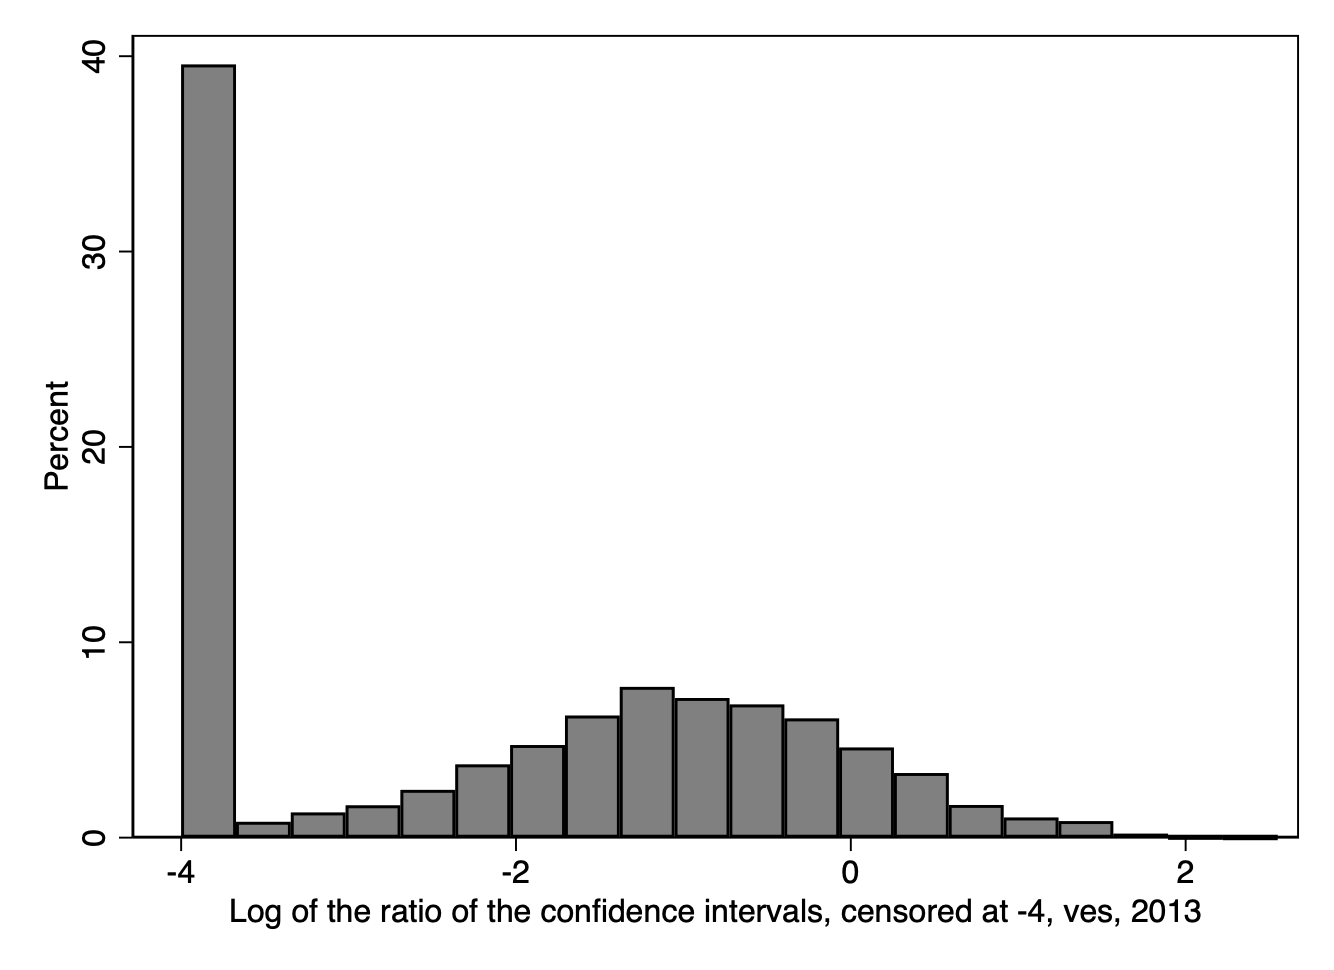
\includegraphics[height=3in]{../../revised_article/comparaison_amplitude_baseline_referee1_2013_ves.png}
    \begin{minipage} [c]  {5in} \scriptsize%
    	    Note: Ratio of the confidence intervals = $ _{}ln(CI_{is}/CI^{ref}_{is})$
    \end{minipage}

    \end{center}
    \end{figure}

   \textbf{XXXX AJouter le complement sur Air et stop XXX} In most cases, the log of the ratio is negative, implying a lower interval confidence of the $\beta$ estimate with our methodology. Our method undoubtedly yields more accurate estimations of the share of additive components, whatever the transport mode considered. We have checked that a similar conclusion applies on other years (they are not reported here for sake of brevity but they are available upon request).
    \end{itemize}

One explanation of the limited accuracy with the alternative method might be the following. Given that the estimation method is run at the country-sector level (exploiting heterogeneity \textit{within} a given country-sector pair), it implicitly assumes that transport costs are independent \textit{across} sectors and \textit{across} origin countries. Put it in plain words, it means that transport costs of say, cars, have nothing in common whether those goods comes from France or from Germany; or that transport costs that apply to imported goods from France have no common component across sectors. One might view this as a disputable assumption. From a statistical point of view further, it implies leaving aside information contained in the fact that transport costs have a both a country-specific component and a sector-specific component, that explains the lower accuracy of the estimation.


\end{itemize}

All these elements, in particular Concern 2 regarding the lower accuracy of the estimates, drive us to maintain our original estimation as benchmark method in the revised version. However, we also want to keep track of this alternative method as further robustness check. For this purpose, we have amended the online Appendix with a section devoted to the referee's method (Section D.3 \textbf{XXX Check XXX}). We deeply hope to convince you of the relevance of this choice.



\subsubsection{Concerns about endogeneity}

\textit{\textbf{The endogeneity problem}: quoting Footnote 14 of the paper, the authors
are estimating $t_i$ and $t_{s(k)}$ as coefficients on the industry or country
dummies times $1/\widetilde{p}_{ik}$. [...] Based on the productivity-sorting model in Melitz (2003) or the quality-sorting
model in Baldwin and Harrigan (2010),  $1/\widetilde{p}_{ik}$ is either positively
or negatively correlated with $\epsilon_{ik}$. So, the NNLS estimates are biased; and
the bias has nothing to with the casual versus accounting interpretation of
the estimates. Accordingly, the one-line justification the authors provide
to not address the endogeneity problem is far from convincing.}

Indeed, this is a very important point. The referee states that, based on theoretical insights by \citet{melitz} or \citet{baldwin_harrigan}, $1/\widetilde{p}_{ik}$ is correlated in one direction on another with residuals $\epsilon_{ik}$. In other words, more productive firms and/or firms selling high-quality products will charge higher prices, all other things equal – in our case, for a given country-product pair.

We obviously do not question this conceptual issue. However, it is worth noting that a good deal of the bias (actually, the part relating to the quality effect) is going to appear identically in the CIF (p) and the FAS ($\widetilde{p}_{ik}$) prices. Consequently, since our dependent variable is based on a ratio between the former and the latter, the (reverse causality) bias cancels out. That said, remains the possibility that bigger firms may impact transport costs, due to their ability of bargaining discounts for larger shipped volumes.

Following the referee's advice, we decided therefore to provide a full set of IV estimates to provide a clean assessment of the size of the potential bias. Section 4.3 in the revised version of the paper provides an overview of the results, while section B.4 in Appendix B provides a full presentation of the theoretical basis for the first-stage equation, as well as first-stage estimates. We follow earlier literature (see e.g. Caliendo and Parro, 2015, or Lashkaripour, 2017) by implementing a first-stage equation regressing $\widetilde{p}$ on custom duties coming based on tariffs at the product line, together with one-year lagged fas prices. First-stage estimates reported in section B.4 show that our main instrumental variable displays the right statistical properties, and that we can confidently re-inject the predictions arising from the first-stage equation for $\widetilde{p}_{ik}$ on the right-hand side of Equation 10 to produce a 2SLS-type of estimation. Figure 9 in the revised version of the paper reports our benchmark estimates by transport mode, together with their instrumented counterpart. In all cases, these estimates are very similar, when not identical. This supports that our benchmark estimates do not suffer any substantial biases arising from endogeneity concerns.

It should be noted that we performed this check on our main dataset (SITC 5 digit), and also at the HS 10 level, to handle simultaneously the referee's concern about aggregation issues. In the latter case, second-stage estimates are not reported for the sake of space, but do not change anything to previous conclusion - they are very, very similar to their non-IV, least squares counterparts. Needless to say that these results are available upon request from the referee.


\subsubsection{The aggregation problem}

\textit{\textbf{The aggregation problem}: The original annual Census data reports
trade at the origin country-HS10 product-district level of aggregation,
whereas the authors are aggregating up the data even further to the origin
country-HS5 industry-year level. Such an aggregation comes with strong implicit assumptions and sacrifices a lot of useful variation in the data.
The authors are motivating the aggregation by stating that the problem
would become computationally expensive without it. But this reasoning
brings us back to my original point that the authors can use the Hummels'
Methodology to circumvent the computational burden.}

It is true that the original annual Census data reports trade at the origin country-HS 10 product-district level of aggregation. Our initial choice of retaining $s=3$ at the sectoral level, $k=5$ at the product level was driven by the use of Hummels' dataset available over 1974-2004 with $k=5$ the finest degree of aggregation. We yet agree with the referee that jumping from $k=10$ to $k=5$ digits at the product level is detrimental to our ability to exploit useful variation in the data. After checking with the US Bureau of Census, HS-10 data is only available since 1989, now available to 2019. As previously mentioned, due to the Covid situation, it was further only possible to receive the data over the years 1997-1999 and from 2001 onwards. In front of this arbitrage, we decided to maintain the case $s=3, k=5$ as baseline, but running estimation at the $s=3,k=10$ in the new Sub-Section 3.3.3 \textbf{XXX CHECK XXX }devoted to robustness analysis.

Additionally, the computational burden mentioned by the referee is not attributable to the product classification level $k=5$ or 10) but rather to the degree of sectoral classification ($s=3$ or 4) as it conditions the number of fixed effects. This explains why we consider the $s=4$ digit- sectoral classification level only for some years. We thank the referee for pointing this ambiguity in our paper, which drove us to rewrite the associated paragraph in the revised version of the paper (see Section 3.3.3 \textbf{XXX CHECK XXX }).


\subsection{Critique 2: Calculation of Unit Prices}

\textit{My second critique concerns the way the authors are calculating the unit prices.
The Census data reports the quantity of goods per observation. So, the authors
can calculate the unit price as Value/Quantity, which is consistent with how
price is modeled in standard trade models. Instead, the authors calculate unit
price as Value/Weight. This used to be a common exercise in the past where
many data-sets did not report Quantity. But, given their data, there is no
justification for the authors to calculate the prices this way.}

\textit{Calculating the unit price as Value/Weight presents the authors
with an additional endogeneity problem. To elaborate, let $\omega_{ik} = Weight/Quantity$
denote the unit weight of the goods in observation $ik$. [...] There is evidence that (i) $\omega_{ik}$ varies significantly within narrowly-defined product
categories, and (ii) $\omega_{ik}$ is negatively correlated with transport costs. So the
way the authors are calculating unit prices and estimating the model creates a
new (but avoidable) source of endogeneity.}

% MEMO: DO NOT FORGET TO REPORT THE ARGUMENTATION BELOW IN THE MAIN TEXT XXX
\paragraph{Our answer:}
\noindent %This is a very important point, and we thank the referee for raising it.
The referee definitely raised a very important point here, and indeed, Census data do report the quantity of goods (and sometimes even two quantities).
%At a more fundamental level, this raises the following question: Do we have reason to believe our measure of unit prices generate significant deviations from the one relying on quantities?
In this context, the findings in \cite{Lashkaripour_JIE2020} are specifically enlightening.
Based on US data very similar to ours over the period 1995-2015, the paper highlights, among other results, that the unit weight of imported goods is indeed substantially heterogeneous even within narrowly-defined product categories and the cost of transportation increases more rapidly with unit weight than the cost of production. \cite{Lashkaripour_JIE2020} finds that accounting for the heterogeneity in export unit weights provides evidence in favor of the iceberg cost assumption regarding transport costs.
This result of transport costs close to be totally iceberg contrasts from our own findings of additive costs representing 30 to 45\% of total costs. Some elements can yet be put forward to account for the difference of results. Beyond a longer time span, our database is exhaustive, and encompasses all goods and industries, while \citet{Lashkaripour_JIE2020}) restricts to indivisible/discrete goods that represent a bit more 56\% of US total imports of goods in his dataset. In this regard, when comparing Tables 1 and 10 in \citet{Lashkaripour_JIE2020}, one can see that the share of multiplicative costs tends to decrease with the share of discrete goods. It is therefore reasonable to think that the inclusion of all goods, like in our setting, would move the average share of multiplicative costs away from 100\%.

Nevertheless, considering the importance of the referee's remark, we went beyond this very first argument to investigate this question in depth. This was not without difficulty yet, in particular due to data and estimation constraints. At a more fundamental level, we also believe that looking at transport costs on a per-weight basis does add relevant information. We develop each line of argument in what follows.

%We now report results based on per-unit prices.
%They confirm the results of \cite{Lashkaripour_JIE2020}
%Yet, first, looking at per-unit prices leads to leaving aside a large part of the data, both sectorally and chronologically.
%Second,  it is interesting to look at additive costs on a per-weight basis even there is a correlation between unit price and weight.

%The two stories are not necessarily incompatible, however.


%Nevertheless, the point made by the referee is an important one and deserves careful investigation. We devoted a lot of thought to a potential switch from weight to quantity.
%Running the estimation considering quantities (i.e., units) rather than weight, still on the transport mode-yearly basis yet appears really uneasy in our context for several, non-trivial reasons, that we develop below.

\subsubsection{Data availability issue}

In our attempt to address the referee's remark, we faced a first difficulty regarding the availability of information on quantities. Neither the US Bureau of Census data nor the 1974-2004 Hummels's data (based on the Census Bureau data) do report the quantity by transport mode. This is incompatible with our empirical strategy of estimation transport costs which is conditional on the transport mode, similarly as in \cite{hummels2007}. As a result, computing the unit price of all trade would require the assumption that the weight per unit is the same for vessel shipments and air shipments at the level of the observation. This is unlikely, as one would expect the higher-to-weight value to be transported by air rather than by vessel. The alternative would then be to only consider single-mode flows. In Hummels's data (1974-2014), on average 41.1 \% of trade flows and 79\% of trade value are multi-mode. This would reduce the total value of the sample from 12,500 billion dollars to 2,650 billion dollars, entailing a large loss of useful information. Original census data, when accessible (from 2002 because of the Covid situation), are more promising.\footnote{Original Census data are  reported at the HS-10 digit $\times$ district of entry $\times$ district of unleading $\times$ rate provision code.} In 2019, multi-modal flows are 570 billion dollars out of 1,790 billion dollars, or 31\% of the data. This is still a large share, but not too large to preclude any work. Accordingly, we dig deeper into this issue with the US Census dataset starting in 2002, restricted to single transport mode flows. \smallskip


The second difficulty dwells on the units used to measure quantities. The Census data, if it provides some information on quantity, remains silent on the units considered. To the best of our knowledge, these can only be found in the ``Harmonized Tariff Schedule of the United State''. Unfortunately, these schedules change many time per year and only the schedules from 2009 onwards were available in a .csv format. On the years for which the match could be done (from 2009), it turns out that at our sector level (3-digit), goods (either at the 5-digit or the 10-digit level) are measured in different units. In 2019, only 125 3-digit sectors out of 230 are measured in a single unit (after cleaning up the unit names\footnote{As units are not always coherent (eg weight can be given in ``kg’’, ``kg.'' ``Kg'' and, also, ``g'' and ``t'').}).\footnote{For instance, 3-digit SITC sector ``061 Sugar, molasses and honey'' includes among other products, 5-digit SITC product ``6150 Molasses, whether or not decolourized'', measured in liters and 5-digit SITC product ``06160 Natural Honey'' measured in kg. Actually worse than this, the 5-digit SITC product ``06190 Other sugars; sugar syrups; artificial honey (whether or not mixed with natural honey); caramel'' includes both 10-digit HTS product ``1702903500 Other: invert molasses'', measured in liters and 10-digit HTS product ``1702602200 Blended syrups described in additional u.s. note 4 to chapter 17: described in general note 15 of the tariff schedule and entered pursuant to its provisions''  measured in kilograms.} Neglecting these differences would invalidate our functional forms, as no one expects the transport cost of a ``piece'' to be the same as the transport cost of a ``kg'', even in the same sector.
So we are limited to using quantity units from 2009 to 2019, amending our structure of fixed effects to consider the triplet (origin country, sector, quantity unit).

\subsubsection{Estimation issue}

Getting deeper on the estimated functional form raised another difficulty in adapting our equation to per-unit rather than per-weight prices. As discussed above, in our baseline regression we separate each transport cost component in its two distinct sector-origin country dimensions. As in \cite{Irrazabal_2015}, we assume an additive form for the additive cost, i.e. $t_{is(k)} = t_i+t_{s(k)}$ with $i$ the origin country and $s$ the sector. In the specific case of quantities, this raises a non-trivial issue for country-level fixed effects. Sector-level fixed effects could indeed be easily replaced by (sector, quantity unit) fixed effects; but the same does not appear relevant for country fixed effects. Let us elaborate on this issue.

In the per-weight price, the existence of a single country fixed effect applicable to all sectors could be justified, as a kilogram is always a kilogram and one can assume they both add the same to transport from, say, Germany. In contrast, an unit of tee-shirt is quite different from an unit of car. To clarify this point, assume imports of tee-shirts and cars from Germany and China. Under the separability assumption, importing a tee-shirt from either country implies paying the fixed effect for both countries (the same for all sectors) and the fixed effect for the sector (the same for all countries); and similarly for importing a car. Hence, the difference in the cost of importing a car from Germany versus China would be the same, in dollars, as the difference between the cost of importing a tee-shirt from Germany relative to China. This does not seem a sensible assumption; in this case specifically, we cannot keep the separability assumption.
As discussed before, this dramatically increases the computational difficulty of our method (with no substantial different results, see Subsection 3.3.1. in the main paper).\smallskip

Integrating these various constraints, we run the robustness check (weight versus quantity) \textit{i)} on a sample reduced over 2009-2019, considering single transport mode flows - amounting to 66\% of the value of the baseline sample; \textit{ii)} retaining a non-separable structure of three-dimensional fixed effects $t_{is(k)u}$, $\tau_{is(k)u}$ according to the following equation:
\begin{equation*}
\ln\left(\frac{p_{iku}}{\widetilde{p}_{iku}}-1 \right)= \ln \left(\tau_{is(k)u} -1+\frac{t_{is(k)u} }{\widetilde{p}_{iku}} \right) + \epsilon_{iku}
\end{equation*}
\noindent where $p_{iku}$ refers to the cif price associated with quantity of goof $k$ imported from country $i$, measured in unit $u$, $\widetilde{p}_{iku}$ the corresponding unit value (fas price). Depending on the sector, two different units are considered, kilograms and numbers.

The results are reported in Table \ref{tab_comp_wgt_qty} and in Figure \ref{graph_comp_wgt_qty} (as well as in the online appendix D.4. In Table \ref{tab_comp_wgt_qty}, for each transport mode, the first column reports the estimation based on the price per quantity; while the second column reports the results obtained considering the price per kg on the same sample; the last column reported our baseline results on the large sample (considering the average value over 2005-2019, under the separability assumption).

\begin{table}[htbp]
	\caption{Comparison: Price per quantity versus per kg, 2009-2019}
	\begin{center}		
		\begin{tabular}{l|ccc|ccc}
\cline{1-7}
Mode: &
  \multicolumn{3}{|c}{Air} &
  \multicolumn{3}{|c}{Vessel} \\ \hline
Price per: & Qy & Kg & Kg & Qy &  Kg & Kg\\ \cline{1-7}
Sample & Limited &Limited  & Baseline & Limited  & Limited & Baseline \\
\hspace{1em}$\#$ of sectors &
22 &22 &216 &60 &60 &225 \\
\hspace{1em}$\#$ of partners &
15 &15 &211 &21 &21 &205 \\
\hspace{1em}$\#$ of pairs &
339 &339 &12,544 &1,100 &1,100 &12,649 \\
\hspace{1em}Trade value (Bn USD)&
242 &
242 &
331 &
583 &
583 &
920 \\ \hline
\multicolumn{7}{l}{Share of additive costs $\beta$} \\ \hline
\hspace{1em} Mean &
0.27 &0.36 &0.22 &0.15 &0.49 &0.45 \\
\hspace{1em} Median &
0.19 &0.16 &0.17 &0.03 &0.51 & 0.44 \\
\hspace{1em} Std. dev. &
0.29 &0.39 &0.19 &0.25 &0.29 &0.26 \\
\hspace{1em} Time trend  coefficient &
-0.049 &-0.054 &-0.026 &0.032 &-0.020 &-0.022 \\ \cline{1-7}
%\multicolumn{1}{l}{beta\_2009} &
%  \multicolumn{1}{|r}{} &
%  \multicolumn{1}{r}{} &
%  \multicolumn{1}{r}{} &
%  \multicolumn{1}{r}{} &
%  \multicolumn{1}{r}{} &
%  \multicolumn{1}{r}{} \\
%\multicolumn{1}{l}{\hspace{1em}Mean} &
%  \multicolumn{1}{|r}{0.33} &
%  \multicolumn{1}{r}{0.47} &
%  \multicolumn{1}{r}{0.23} &
%  \multicolumn{1}{r}{0.14} &
%  \multicolumn{1}{r}{0.51} &
%  \multicolumn{1}{r}{0.48} \\
%\multicolumn{1}{l}{beta\_2019} &
%  \multicolumn{1}{|r}{} &
%  \multicolumn{1}{r}{} &
%  \multicolumn{1}{r}{} &
%  \multicolumn{1}{r}{} &
%  \multicolumn{1}{r}{} &
%  \multicolumn{1}{r}{} \\
%\multicolumn{1}{l}{\hspace{1em}Mean} &
%  \multicolumn{1}{|r}{0.21} &
%  \multicolumn{1}{r}{0.31} &
%  \multicolumn{1}{r}{0.19} &
%  \multicolumn{1}{r}{0.17} &
%  \multicolumn{1}{r}{0.44} &
%  \multicolumn{1}{r}{0.50} \\
\end{tabular}

%		\begin{tabular}{lllllll}
\cline{1-7}
\multicolumn{1}{c}{} &
  \multicolumn{3}{|c}{air} &
  \multicolumn{3}{c}{ves} \\
\multicolumn{1}{c}{} &
  \multicolumn{1}{|r}{hs10\_qy1\_qy} &
  \multicolumn{1}{r}{hs10\_qy1\_wgt} &
  \multicolumn{1}{r}{baseline} &
  \multicolumn{1}{r}{hs10\_qy1\_qy} &
  \multicolumn{1}{r}{hs10\_qy1\_wgt} &
  \multicolumn{1}{r}{baseline} \\
\cline{1-7}
\multicolumn{1}{l}{Mean} &
  \multicolumn{1}{|r}{} &
  \multicolumn{1}{r}{} &
  \multicolumn{1}{r}{} &
  \multicolumn{1}{r}{} &
  \multicolumn{1}{r}{} &
  \multicolumn{1}{r}{} \\
\multicolumn{1}{l}{\hspace{1em}Nb\_sectors} &
  \multicolumn{1}{|r}{216} &
  \multicolumn{1}{r}{217} &
  \multicolumn{1}{r}{217} &
  \multicolumn{1}{r}{223} &
  \multicolumn{1}{r}{226} &
  \multicolumn{1}{r}{226} \\
\multicolumn{1}{l}{\hspace{1em}Nb\_partners} &
  \multicolumn{1}{|r}{207} &
  \multicolumn{1}{r}{210} &
  \multicolumn{1}{r}{210} &
  \multicolumn{1}{r}{204} &
  \multicolumn{1}{r}{205} &
  \multicolumn{1}{r}{205} \\
\multicolumn{1}{l}{\hspace{1em}Nb\_pairs} &
  \multicolumn{1}{|r}{11,210} &
  \multicolumn{1}{r}{12,461} &
  \multicolumn{1}{r}{12,461} &
  \multicolumn{1}{r}{11,931} &
  \multicolumn{1}{r}{12,656} &
  \multicolumn{1}{r}{12,656} \\
\multicolumn{1}{l}{\hspace{1em}Covered trade value} &
  \multicolumn{1}{|r}{3.01e+11} &
  \multicolumn{1}{r}{3.23e+11} &
  \multicolumn{1}{r}{3.23e+11} &
  \multicolumn{1}{r}{8.98e+11} &
  \multicolumn{1}{r}{9.18e+11} &
  \multicolumn{1}{r}{9.18e+11} \\
\multicolumn{1}{l}{beta} &
  \multicolumn{1}{|r}{} &
  \multicolumn{1}{r}{} &
  \multicolumn{1}{r}{} &
  \multicolumn{1}{r}{} &
  \multicolumn{1}{r}{} &
  \multicolumn{1}{r}{} \\
\multicolumn{1}{l}{\hspace{1em}Mean} &
  \multicolumn{1}{|r}{0.05} &
  \multicolumn{1}{r}{0.23} &
  \multicolumn{1}{r}{0.23} &
  \multicolumn{1}{r}{0.21} &
  \multicolumn{1}{r}{0.45} &
  \multicolumn{1}{r}{0.47} \\
\multicolumn{1}{l}{\hspace{1em}Median} &
  \multicolumn{1}{|r}{0.00} &
  \multicolumn{1}{r}{0.18} &
  \multicolumn{1}{r}{0.19} &
  \multicolumn{1}{r}{0.05} &
  \multicolumn{1}{r}{0.44} &
  \multicolumn{1}{r}{0.45} \\
\multicolumn{1}{l}{\hspace{1em}Std. dev.} &
  \multicolumn{1}{|r}{0.12} &
  \multicolumn{1}{r}{0.20} &
  \multicolumn{1}{r}{0.19} &
  \multicolumn{1}{r}{0.28} &
  \multicolumn{1}{r}{0.25} &
  \multicolumn{1}{r}{0.27} \\
\multicolumn{1}{l}{Time trend} &
  \multicolumn{1}{|r}{} &
  \multicolumn{1}{r}{} &
  \multicolumn{1}{r}{} &
  \multicolumn{1}{r}{} &
  \multicolumn{1}{r}{} &
  \multicolumn{1}{r}{} \\
\multicolumn{1}{l}{\hspace{1em}Coefficient} &
  \multicolumn{1}{|r}{-0.073} &
  \multicolumn{1}{r}{-0.059} &
  \multicolumn{1}{r}{-0.061} &
  \multicolumn{1}{r}{-0.354} &
  \multicolumn{1}{r}{-0.059} &
  \multicolumn{1}{r}{-0.066} \\
\multicolumn{1}{l}{beta\_2005} &
  \multicolumn{1}{|r}{} &
  \multicolumn{1}{r}{} &
  \multicolumn{1}{r}{} &
  \multicolumn{1}{r}{} &
  \multicolumn{1}{r}{} &
  \multicolumn{1}{r}{} \\
\multicolumn{1}{l}{\hspace{1em}Mean} &
  \multicolumn{1}{|r}{0.04} &
  \multicolumn{1}{r}{0.30} &
  \multicolumn{1}{r}{0.29} &
  \multicolumn{1}{r}{0.27} &
  \multicolumn{1}{r}{0.50} &
  \multicolumn{1}{r}{0.53} \\
\multicolumn{1}{l}{beta\_2019} &
  \multicolumn{1}{|r}{} &
  \multicolumn{1}{r}{} &
  \multicolumn{1}{r}{} &
  \multicolumn{1}{r}{} &
  \multicolumn{1}{r}{} &
  \multicolumn{1}{r}{} \\
\multicolumn{1}{l}{\hspace{1em}Mean} &
  \multicolumn{1}{|r}{0.04} &
  \multicolumn{1}{r}{0.20} &
  \multicolumn{1}{r}{0.19} &
  \multicolumn{1}{r}{0.25} &
  \multicolumn{1}{r}{0.50} &
  \multicolumn{1}{r}{0.50} \\
\cline{1-7}
\end{tabular}

{\parbox[l]{12cm}{ \vspace{4pt}\footnotesize{Notes: Time trend coefficient is the annual growth rate.}}}
\end{center}
	\label{tab_comp_wgt_qty}%
\end{table}%

\begin{figure}[htbp]
	\caption{$\beta$ Estimate: Price per quantity or price per kg, 2009-2019}
	\begin{center}
		\begin{tabular}{cc}
			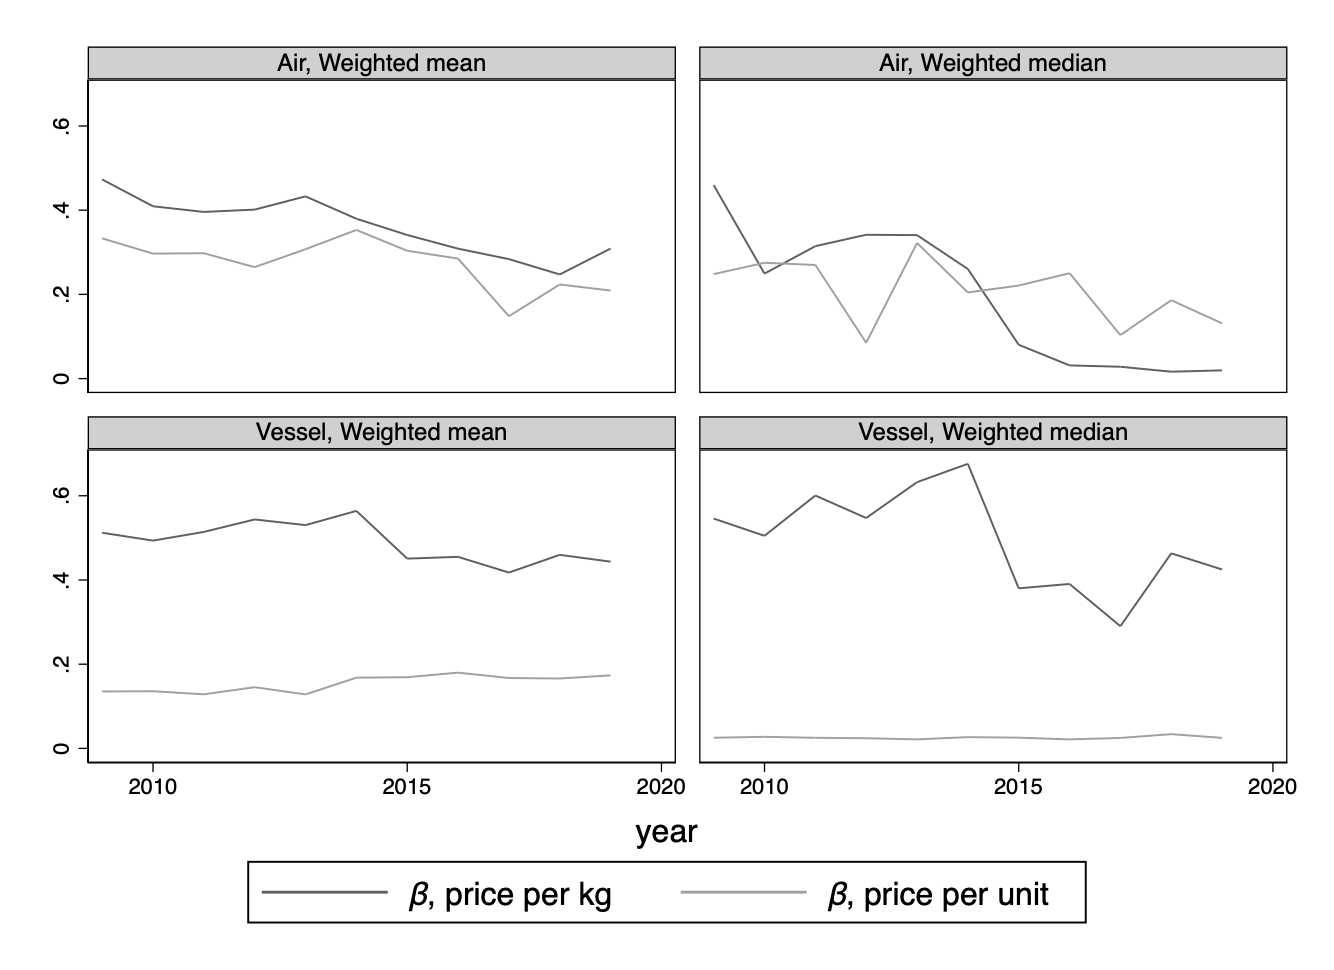
\includegraphics[height=8cm]{../../revised_article/scatter_chronology_non_separe_wgt_non_separe_qy.png}\\
			\multicolumn{2}{l}{{\footnotesize Notes: In both cases, estimation is run without imposing the separability assumption.}}
		\end{tabular}
	\end{center}
		\label{graph_comp_wgt_qty}%
\end{figure}

Two main results emerge. First, given the constraints on the sample selection for quantities, the estimation based on quantity can only be run on a reduced sample. In contrast to the aggregation and the separability issues, these restrictions that strongly limit both the number of sectors and of countries covered, do also impact the value of trade flows covered. In our view, this raises a non-trivial sample selection bias that may reduce the general scope of the transport cost estimates. Second, in terms of $\beta$ estimates, the results show clearly that using price per unit (whatever that unit is) instead of price per weight decreases the share of additive costs (except if one look at the median for air). In this regard, they stand in line with the results of \cite{Lashkaripour_JIE2020}, stressing the correlation between weight per unit and unit price. Still, the share of additive cost is not reduced to zero (except if one looks at the median for vessel). Thus these results do not disqualify our approach, especially as we cover a much larger period and sample with our baseline estimate.

\subsubsection{On the relevance of the price per-weight approach}
At a more fundamental level, we do believe that the study of transport costs measured on a per-weight price add some relevant information on the international transport cost burden faced by exporters. Let us explain the underlying rationale.

Our main objective in this paper is to provide a quantitative assessment of the international transport costs burden over time; on that matter, one may start with the observation that transport cost schedules are expressed through a mixed, per-weight and per-volume basis, both historically and nowadays. For example, in 2021, air freight trade costs are expressed in weights, with a minimal weight per volume (``volumetric weight'' or ``dimensional weight'')\footnote{See for example \href{https://transporteca.co.uk/shipping-costs}{https://transporteca.co.uk/shipping-costs}, \href{http://wap.dhl.com/serv/volweight.html}{http://wap.dhl.com/serv/volweight.html} and \href{https://en.wikipedia.org/wiki/Dimensional_weight}{ https://en.wikipedia.org/wiki/Dimensional\_weight}).} while maritime freight costs are expressed in volume.
Hence, looking at per-kg transport cost can be interpreted straightforwardly as trying to estimate the actual existing shipping costs, with sector fixed effects interpretable as measure of mean density for different sectors. The existence of per-volume or per-weight shipping cost is directly linked to the technical constraints of the transportation sector, hence exogenous to exporting firms' decisions. In contrast, per-unit shipping cost depends on the behavior of exporting firms. The shipping cost per weight is one of the exogenous parameters firms take into account in their production choices, including weight per unit. Accordingly, studying the technical per-volume or per-weight shipping cost is interesting to understand the context in which they operate.

Another argument is illustrated by Figure \ref{graph_Share_of_discrete_goods.png}. After computing the share of discrete goods per 5-digit SITC import in 2009, we have used the changing composition of US imports to approximate the share of discrete goods in the total value of US imports on a yearly basis. According to this rough approximation, discrete goods are between 23\% and 52\% of US imports, reaching a value only above 50\% for two years. Switching to a per-unit approach would hence mean a marked reduction in the trade flows coverage, thereby limiting the general scope of our estimates.


\begin{figure}[htbp]
	\caption{Estimated share of discrete goods in US imports, 1974-2019}
	\begin{center}
		\begin{tabular}{cc}
			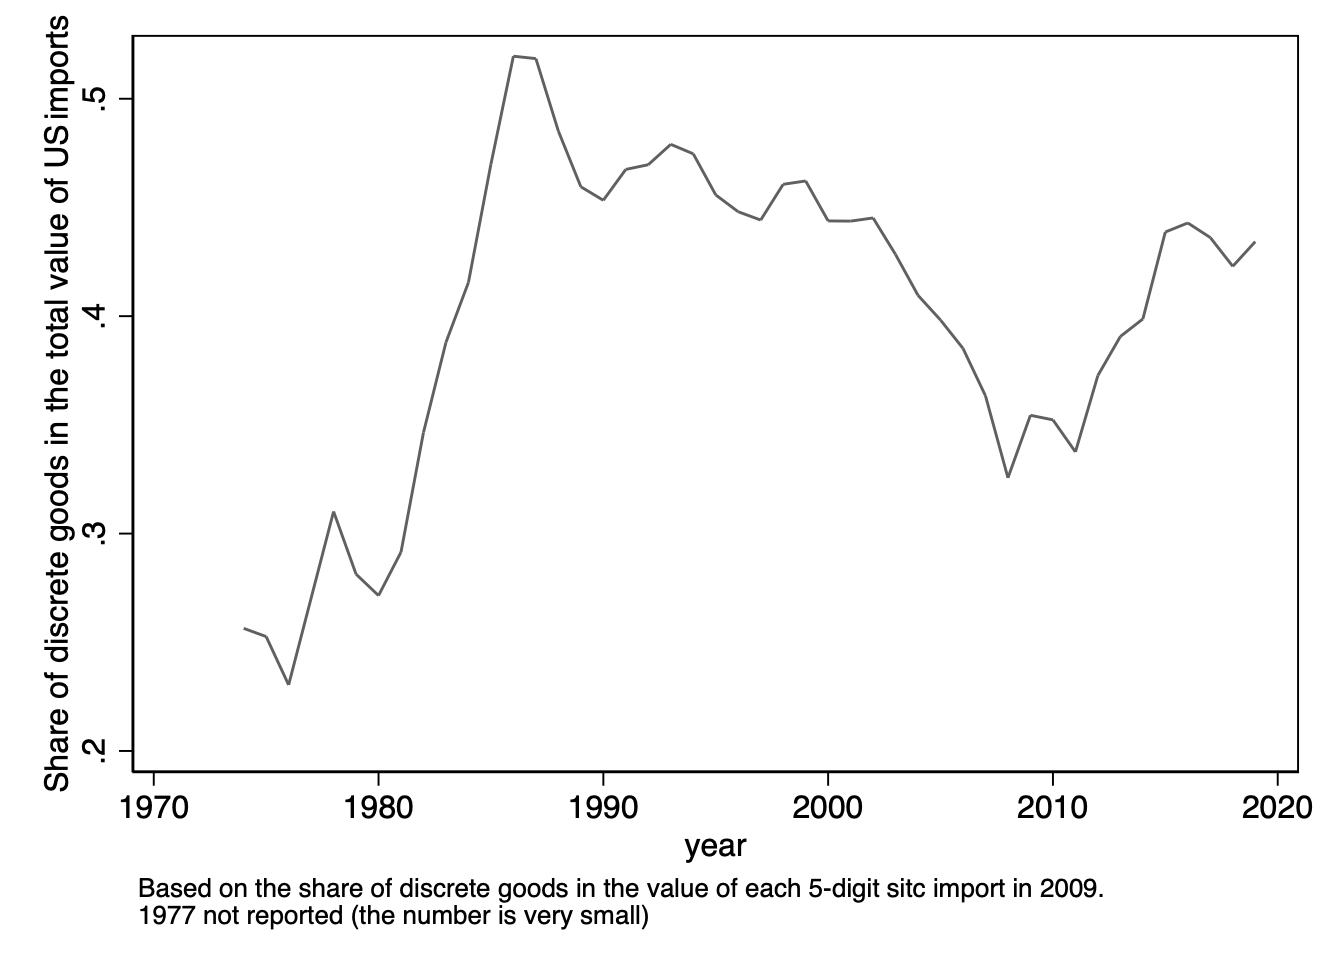
\includegraphics[height=8cm]{../../revised_article/Share_of_discrete_goods.png}\\
		\end{tabular}
	\end{center}
	\label{graph_Share_of_discrete_goods.png}%
\end{figure}


After considering all the above arguments in depth, we decided not to switch the paper from the study of price per weight to the study of price per quantity. We thus maintained our original empirical strategy covering the whole period 1974-2019 in the revised version, while we extended the online Appendix with this supplementary robustness check. We hope to have convinced you that this is a relevant choice.

\subsection{Critique 3: Big Picture Implications}

\textit{My third critique concerns the lack of an exciting punchline. The fact that
composition effects have not countervailed the reduction in pure transport costs
(at least not as much as previously believed) is an interesting but minor observation.
Does this observation revise our understanding of say the gains from
trade? Does it shed new light on a puzzle many people are thinking about?
One crude suggestion is to see how the reduction in the industry-specific cost
terms is related to the industry-level trade elasticities. If the composition effects
favor low-elasticity industries, the findings in the paper may have first-order
implications for the gains from trade.
Another suggestion is to dig deeper into the relative rate at which additive
and multiplicative transport costs have declined over time. Since additive transport
costs favor rich (high-quality exporting) countries, the disproportionally
greater reduction in additive costs can perhaps explain the rise of low-income
exporter as documented by Hanson (2012, JEP).}

\paragraph{Our answer:}
\noindent We devoted a lot of thought to this point, which directly echoed a similar concern by the other referee. Taking stock of your suggestion, we decided to offer insights on the welfare implications of our results. In this regard, the new section 5 ``The role of additive cost: Theoretical insights'' is devoted to a theory-based analysis of the alterations to welfare gains involved by the relative variations of additive and multiplicative transport costs over our period of analysis. To do so, we start from the canonical \cites{melitz} model where we add additive trade costs. The inclusion of additive costs in a \citet{melitz} setting has already been performed in \citet{sorensen2014} and \citet{Irrazabal_2015}. However, \citet{sorensen2014} exclusively performs a theoretical analysis, without any quantitative exercise. In addition to a partial equilibrium extension of \citet{melitz}, \citet{Irrazabal_2015} do perform a quantitative simulation to assess the welfare variations induced by the presence of additive costs, but the latter is based on a calibration for transport costs restricted to 2004, based on the case of Nowrway. In contrast, our own exercise relies on a several decades time span for the US, allowing us to highlight the welfare alterations induced over time by the relative dynamics of additive and multiplicative costs, based on ``true'' values for the latter - remember that our methodology allows for the identification of both multiplicative and additive costs as a share of total costs, whereas additive costs in \citet{Irrazabal_2015} are expressed relatively to the (median) export price.

More precisely, we use some of the estimates underlying results reported in Section 3 concerning multiplicative and additive costs, more precisely those for the years 1974 and 2019. Based on the latter, we implement several comparative statics exercises to investigate the different welfare consequences of alterations to multiplicative and additive costs. In addition, we also assess how the latter results are distorted by changes in sunk costs of exports, $f_{x}$. To that end, we adjust the share of exporting firms in the US: Based on \citet{Lincoln_McCallum2018}, we set the latter to 35\% in 2019, versus 21\% in 1974. In our preferred exercise, we quantify the welfare gains that derive from the reduction in transport costs as documented in Section 3, relying on a combined reduction in each additive/iceberg component, with the reduction in the fixed export cost. We compare this with the case where the total transport costs reduction is solely attributed to a decrease in ad-valorem costs.

Table 5 in Section 5 of the paper reports the results of these various comparative statics exercises for Air and Vessel transport modes. Specifically, we report the change in total transport costs decomposed in its two dimensions (additive and ad-valorem); as well as the welfare change, both in absolute and in relative terms. Qualitatively, the conclusions are identical for both transport modes, with two major insights. First, for a given decrease in total transport costs,  welfare gains are around 50\% higher when this reduction is partly achieved through a reduction in the additive costs. Second, the decrease in export sunk costs (i.e., increase in the share of exporting firms) proportionally amplifies the gains from decreasing variable costs, with again an additional premium coming from the decrease of additive costs.

Overall, these results appear to add a substantial contribution to the paper : We are able to provide a quantitative assessment of the welfare gains induced by the decrease in both types (additive and multiplicative) of costs over a 45-year period, and to highlight the respective part of each component in the determination of these gains. Note also that not only the inclusion of additive costs in the underlying framework generates large welfare differences, but also that the latter are probably a lower bound of the welfare variations induced by changes in additive \emph{trade} costs, larger than the sole transport costs.



%XXX is chosen to match the share of firms exporting in Norway (38 percent, Moxnes, 2010), while

%IMO : The data cover all Norwegian non-oil exporters in 2004 and originate from customs declarations.



%\textbf{Comments about that}

%\paragraph{Piste 1} Consider his/her first suggestion. What is the idea? First, the link between gains from trade and trade-elasticity. Am I correct in saying that gains from trade are higher when trade is about low-elasticity goods? The idea being, if national goods are low substitutes, then here are larger gains from trading them. So, if composition effects (trade shifts between sectors) favor low-elasticity sectors, then one might expect high gains from trade. Hummels: trade composition effects matter as they partially offset the reduction in pure transport costs for both air and vessel. Over time, tendency to trade goods more costly to export everything else equal. So, if the referee's assertion is right (trade composition effects favor low-elasticity sectors), then increasing gains from trade. But, we disagree with Hummels' findings (his way of measuring things is inappropriate) and find that trade composition effects do not matter much, at least for air (for vessel, the composition effects matter more, but by amplifying the reduction in transport costs, ie towards goods that are less costly to export). Meaning that gains from trade are purely due to reduction in transport costs at the sector, but not from switch towards low-elasticity sectors. Identify one source of gains from trade, not two.

%What to do with this? When composition effects do matter (ocean freight), do they favor low-elasticity industries? In which case, on top of the reduction in transport costs per se (which has welfare consequences as well), one might expect additional gains from these composition effects. When they don't, this mitigates the gains from trade that could be expected from the picture given by Hummels.

%\textbf{GD20200708 Hum... Je crois que je comprends le point dur referee et je suis d’accord avec lui. Le souci, c’est que de toutes les manières, je ne sais pas si cela favorise les high ou les low elasticity. Mais on pourrait voir.}

%\paragraph{Piste 2} What is at stake? Show that how $\beta$ = the relative share of additive costs has evolved over time. Good idea as this is really what differentiates us from Hummels, model a varying $\beta$ over time. Specifically, how methodology lets the $\beta$ vary over the three time-sector-partner country dimension. Show how $\beta$ varies over time everything else equal? Hopefully, goes in the referee's direction (decreases over time) with possibly a role in the understanding in the ``big picture'' of trade patterns?

%\paragraph{Piste 3} \textbf{GD20200708 On sait que les additive costs sont plus distorsifs que les multiplicative costs, puisqu’ils modifient les prix relatifs. Donc le fait qu’ils sont une partie croissante des costs signifie qu’on sur-estime l’augmentation des gains de welfare liés à la baisse des coûts de transport}

%\newpage
\bibliographystyle{apalike2}
\bibliography{biblio}


\end{document}

